\documentclass{standalone}

\usepackage[english]{babel}
\usepackage[utf8x]{inputenc}
\usepackage[T1]{fontenc}
\usepackage{tikz,pgf} %and any other packages or tikzlibraries your picture needs
\usepackage{amsfonts}
\usepackage{amsmath}
\usepackage{physics}
\usepackage{amssymb}
\usepackage{mathtools}
\usetikzlibrary{shapes,arrows,patterns}

\begin{document}

%%%%%%%%%%%%%%%%%%%%%%%%%%%%%%%%%%%%%%%%%%%%%%%%%%%%%%%%%%%%%%%%%%%%%%%%%%%%%%%%
%COPY HERE
%%%%%%%%%%%%%%%%%%%%%%%%%%%%%%%%%%%%%%%%%%%%%%%%%%%%%%%%%%%%%%%%%%%%%%%%%%%%%%%%


\tikzset{every picture/.style={line width=0.75pt}} %set default line width to 0.75pt

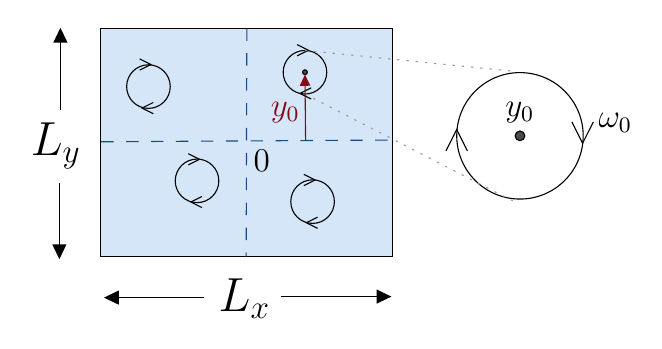
\begin{tikzpicture}[x=0.75pt,y=0.75pt,yscale=-1,xscale=1]
%uncomment if require: \path (0,300); %set diagram left start at 0, and has height of 300

%Shape: Rectangle [id:dp8537790588861109]
\draw  [fill={rgb, 255:red, 214; green, 230; blue, 249 }  ,fill opacity=1 ] (49.92,61.08) -- (190.42,61.08) -- (190.42,171.08) -- (49.92,171.08) -- cycle ;
%Straight Lines [id:da2934066429939679]
\draw    (30,135.75) -- (30,169.25) ;
\draw [shift={(30,172.25)}, rotate = 270] [fill={rgb, 255:red, 0; green, 0; blue, 0 }  ][line width=0.08]  [draw opacity=0] (7.14,-3.43) -- (0,0) -- (7.14,3.43) -- cycle    ;
%Straight Lines [id:da8241212049271052]
\draw    (30.5,100.25) -- (30.5,63.75) ;
\draw [shift={(30.5,60.75)}, rotate = 450] [fill={rgb, 255:red, 0; green, 0; blue, 0 }  ][line width=0.08]  [draw opacity=0] (7.14,-3.43) -- (0,0) -- (7.14,3.43) -- cycle    ;
%Straight Lines [id:da8954416056914352]
\draw    (137,190.25) -- (187,190.25) ;
\draw [shift={(190,190.25)}, rotate = 180] [fill={rgb, 255:red, 0; green, 0; blue, 0 }  ][line width=0.08]  [draw opacity=0] (7.14,-3.43) -- (0,0) -- (7.14,3.43) -- cycle    ;
%Straight Lines [id:da9428515181591588]
\draw    (99.5,190.75) -- (54.5,190.75) ;
\draw [shift={(51.5,190.75)}, rotate = 360] [fill={rgb, 255:red, 0; green, 0; blue, 0 }  ][line width=0.08]  [draw opacity=0] (7.14,-3.43) -- (0,0) -- (7.14,3.43) -- cycle    ;
%Shape: Circle [id:dp878186290771406]
\draw   (137.83,82.17) .. controls (137.83,76.37) and (142.53,71.67) .. (148.33,71.67) .. controls (154.13,71.67) and (158.83,76.37) .. (158.83,82.17) .. controls (158.83,87.97) and (154.13,92.67) .. (148.33,92.67) .. controls (142.53,92.67) and (137.83,87.97) .. (137.83,82.17) -- cycle ;
\draw   (144.53,68.87) -- (149.93,71.57) -- (144.53,74.27) ;
\draw   (151.33,95.07) -- (145.93,92.37) -- (151.33,89.67) ;

%Shape: Circle [id:dp37751711035932245]
\draw   (62.42,89.08) .. controls (62.42,83.28) and (67.12,78.58) .. (72.92,78.58) .. controls (78.72,78.58) and (83.42,83.28) .. (83.42,89.08) .. controls (83.42,94.88) and (78.72,99.58) .. (72.92,99.58) .. controls (67.12,99.58) and (62.42,94.88) .. (62.42,89.08) -- cycle ;
\draw   (68.67,75.73) -- (74.07,78.43) -- (68.67,81.13) ;
\draw   (75.27,102.13) -- (69.87,99.43) -- (75.27,96.73) ;

%Shape: Circle [id:dp9441129857051875]
\draw   (141.5,144.5) .. controls (141.5,138.7) and (146.2,134) .. (152,134) .. controls (157.8,134) and (162.5,138.7) .. (162.5,144.5) .. controls (162.5,150.3) and (157.8,155) .. (152,155) .. controls (146.2,155) and (141.5,150.3) .. (141.5,144.5) -- cycle ;
\draw   (147.8,131.4) -- (153.2,134.1) -- (147.8,136.8) ;
\draw   (154.4,157.4) -- (149,154.7) -- (154.4,152) ;

%Shape: Ellipse [id:dp23625262988639273]
\draw   (221.46,112.8) .. controls (221.46,95.98) and (235.1,82.34) .. (251.92,82.34) .. controls (268.74,82.34) and (282.38,95.98) .. (282.38,112.8) .. controls (282.38,129.62) and (268.74,143.26) .. (251.92,143.26) .. controls (235.1,143.26) and (221.46,129.62) .. (221.46,112.8) -- cycle ;
\draw   (287.26,106.08) -- (282.09,116.41) -- (276.93,106.08) ;
%Shape: Circle [id:dp7990969910924739]
\draw  [fill={rgb, 255:red, 74; green, 74; blue, 74 }  ,fill opacity=1 ] (249.59,112.8) .. controls (249.59,111.51) and (250.63,110.47) .. (251.92,110.47) .. controls (253.21,110.47) and (254.26,111.51) .. (254.26,112.8) .. controls (254.26,114.09) and (253.21,115.14) .. (251.92,115.14) .. controls (250.63,115.14) and (249.59,114.09) .. (249.59,112.8) -- cycle ;
\draw   (216.26,120.07) -- (221.43,109.75) -- (226.59,120.07) ;
%Straight Lines [id:da01276353140729447]
\draw [color={rgb, 255:red, 155; green, 155; blue, 155 }  ,draw opacity=1 ] [dash pattern={on 0.84pt off 2.51pt}]  (148.33,71.67) -- (250.43,81.86) ;
%Straight Lines [id:da5308408420530641]
\draw [color={rgb, 255:red, 155; green, 155; blue, 155 }  ,draw opacity=1 ] [dash pattern={on 0.84pt off 2.51pt}]  (148.33,92.67) -- (248.43,144.14) ;
%Shape: Circle [id:dp1732750756124548]
\draw   (85.83,134.5) .. controls (85.83,128.7) and (90.53,124) .. (96.33,124) .. controls (102.13,124) and (106.83,128.7) .. (106.83,134.5) .. controls (106.83,140.3) and (102.13,145) .. (96.33,145) .. controls (90.53,145) and (85.83,140.3) .. (85.83,134.5) -- cycle ;
\draw   (92.13,121.4) -- (97.53,124.1) -- (92.13,126.8) ;
\draw   (98.73,147.4) -- (93.33,144.7) -- (98.73,142) ;

%Straight Lines [id:da29014475525837846]
\draw [color={rgb, 255:red, 23; green, 74; blue, 133 }  ,draw opacity=1 ] [dash pattern={on 4.5pt off 4.5pt}]  (120.33,61) -- (120,171.17) ;
%Straight Lines [id:da393091957111789]
\draw [color={rgb, 255:red, 23; green, 74; blue, 133 }  ,draw opacity=1 ] [dash pattern={on 4.5pt off 4.5pt}]  (50.17,115.67) -- (190.33,114.83) ;
%Shape: Circle [id:dp6141644536349495]
\draw  [fill={rgb, 255:red, 74; green, 74; blue, 74 }  ,fill opacity=1 ] (147.17,82.17) .. controls (147.17,81.52) and (147.69,81) .. (148.33,81) .. controls (148.98,81) and (149.5,81.52) .. (149.5,82.17) .. controls (149.5,82.81) and (148.98,83.33) .. (148.33,83.33) .. controls (147.69,83.33) and (147.17,82.81) .. (147.17,82.17) -- cycle ;
%Straight Lines [id:da09330324548659452]
\draw [color={rgb, 255:red, 128; green, 10; blue, 25 }  ,draw opacity=1 ]   (148.63,114.94) -- (148.36,86.33) ;
\draw [shift={(148.33,83.33)}, rotate = 449.47] [fill={rgb, 255:red, 128; green, 10; blue, 25 }  ,fill opacity=1 ][line width=0.08]  [draw opacity=0] (5.36,-2.57) -- (0,0) -- (5.36,2.57) -- cycle    ;

% Text Node
\draw (105.5,180.4) node [anchor=north west][inner sep=0.75pt]  [font=\LARGE]  {$L_{x}$};
% Text Node
\draw (15,105.4) node [anchor=north west][inner sep=0.75pt]  [font=\LARGE]  {$L_{y}$};
% Text Node
\draw (243.59,95.54) node [anchor=north west][inner sep=0.75pt]  [font=\large]  {$y_{0}$};
% Text Node
\draw (130.59,95.54) node [anchor=north west][inner sep=0.75pt]  [font=\large,color={rgb, 255:red, 128; green, 10; blue, 25 }  ,opacity=1 ]  {$y_{0}$};
% Text Node
\draw (122.3,118.25) node [anchor=north west][inner sep=0.75pt]  [font=\large]  {$0$};
% Text Node
\draw (288.59,100.54) node [anchor=north west][inner sep=0.75pt]  [font=\large]  {$\omega _{0}$};


\end{tikzpicture}


%%%%%%%%%%%%%%%%%%%%%%%%%%%%%%%%%%%%%%%%%%%%%%%%%%%%%%%%%%%%%%%%%%%%%%%%%%%%%%%%
%COPY HERE
%%%%%%%%%%%%%%%%%%%%%%%%%%%%%%%%%%%%%%%%%%%%%%%%%%%%%%%%%%%%%%%%%%%%%%%%%%%%%%%%

\end{document}
